\section{Acceleration}
Rendering the triangle meshes quickly becomes a time intensive task, if the triangles forming the model are stored in a simple list. For example the scene shown in figure~\ref{fig:teapot} consists of the Utah teapot standing on a plane, illuminated by a point light. Rendering it without an acceleration structure with enabled shadows takes approximately 1151 seconds or 19 minutes and 11 seconds. A first measure to improve matters is to surround the mesh with a box. Only if an incoming ray hits the box is it intersected with the triangles of the mesh. Using a bounding box reduces the rendering time to 613 seconds or about 10 min for scene~\ref{fig:teapot}. To reduce computations required to render the scene further the number of intersection tests per pixel has to be reduced further. This can be done by subdividing the bounding box. Three different ways if subdivision will be considered. All of the start by finding the longest dimension of the box, but differ in the way this longest dimension is split. The first method splits the parent box into two children in the geometric middle of the longest axis. The second method sorts the triangles contained in the box according to their centroid coordinate of the axis under consideration. Finally the surface area heuristic is considered, which splits along several points and chooses the best one. Table~\ref{tab:teapodTiming} shows the timing results of the three implemented splitting methods.

\begin{table}
\centering
\begin{tabular}{|c|c|c|c|c|} \hline
				& read[s] & split[s] & render[s] & total[s] \\ \hline
Middle-Split    & 0.16 & 0.95  & 23.61  & 24.72	\\
Sort-Split      & 0.17 & 0.06  & 30.47  & 30.7	\\
SAH             & 0.16 & 0.18  & 17.27  & 17.61	\\ \hline
\end{tabular}
\caption{Time measurments taken using various splitting methods when rendering the teapot scene.}
\label{tab:teapodTiming}
\end{table}

\begin{figure}
\centering
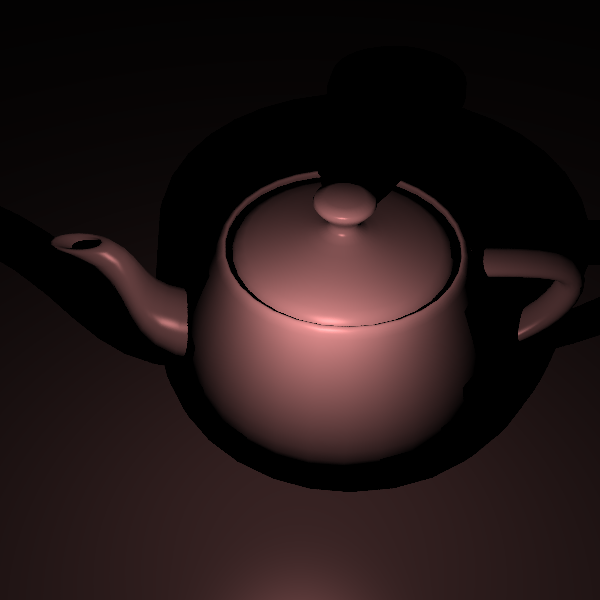
\includegraphics[width=0.45\linewidth]{./img/teapot}
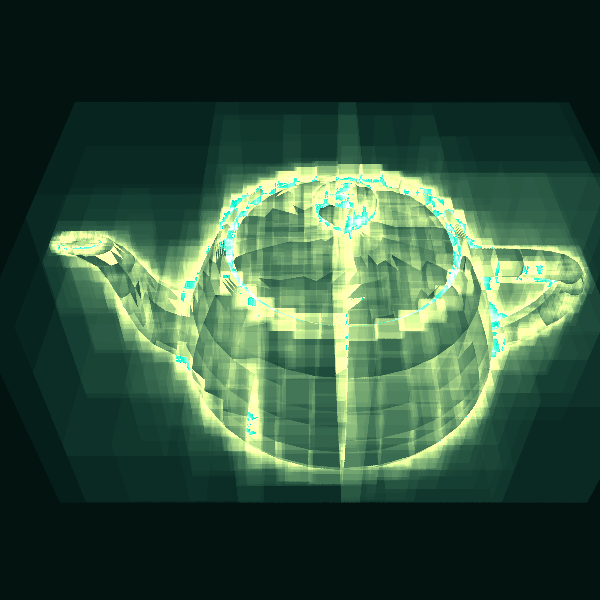
\includegraphics[width=0.45\linewidth]{./img/teaFCGreen10}
\caption{Utah-Teapot rendered image and false color visualizations of the intersections with a color map maximum at 180 intersections, with 10 SAH cuts per split.}
\label{fig:teapotWithAcc}
\end{figure}

\begin{table}
\centering
\begin{tabular}{|c|c|c|c|c|} \hline
				& read[s] & split[s] & render[s] & total[s] \\ \hline
Middle-Split    & 11.4 & 3.7   &  10.53  & 25.63 \\
Sort-Split      & 10.6 & 4.6   &  20.5  & 35.7	 \\
SAH             & 11.0 & 14.3  &  6.71  & 32.01	 \\ \hline
\end{tabular}
\caption{Time measurments taken using various splitting methods when rendering the stanford dragon scene.}
\label{tab:DragonTiming}
\end{table}


\begin{figure}
\centering
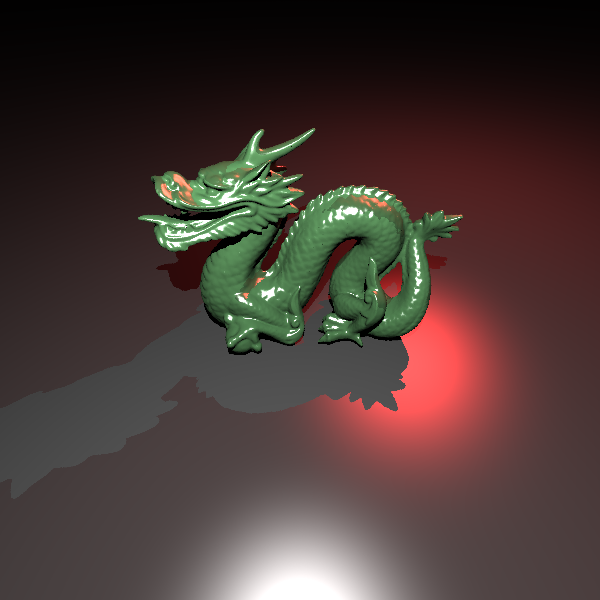
\includegraphics[width=0.45\linewidth]{./img/dragon}
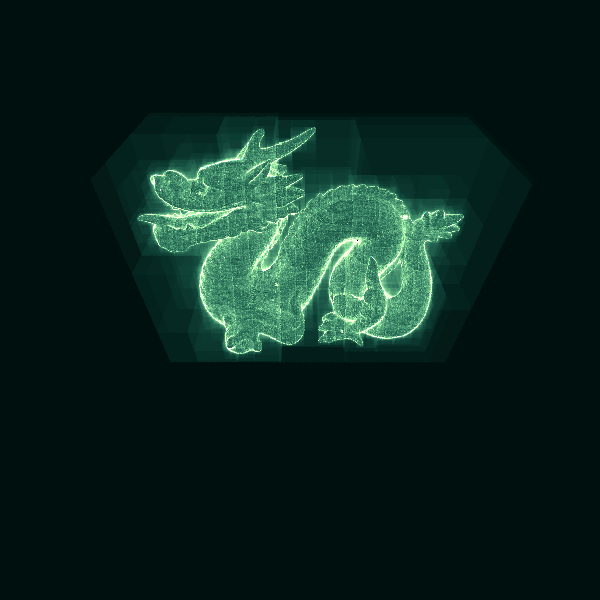
\includegraphics[width=0.45\linewidth]{./img/dragonFC4}
\caption{High resolution Standford-Dragon rendered image and false color visualizations of the intersections with a color map maximum at 180 intersections and 4 SAH cuts per split }
\label{fig:dragon}
\end{figure}


\section{Textures}

\begin{figure}
\centering
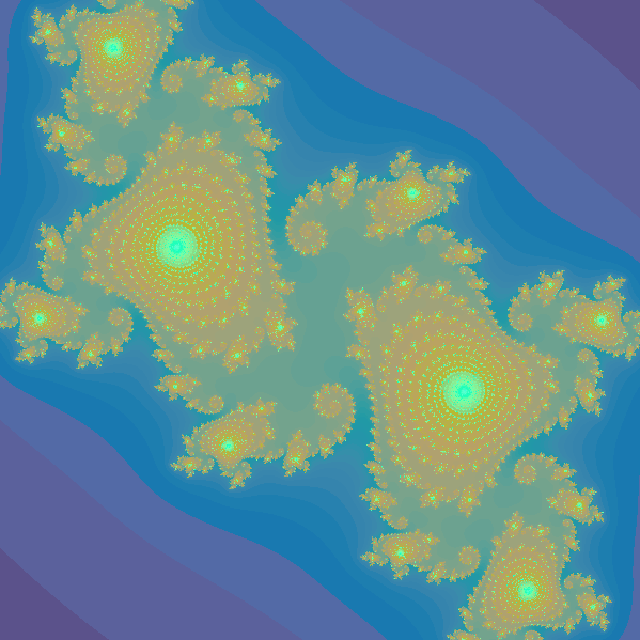
\includegraphics[width=0.26\linewidth]{./img/julia}
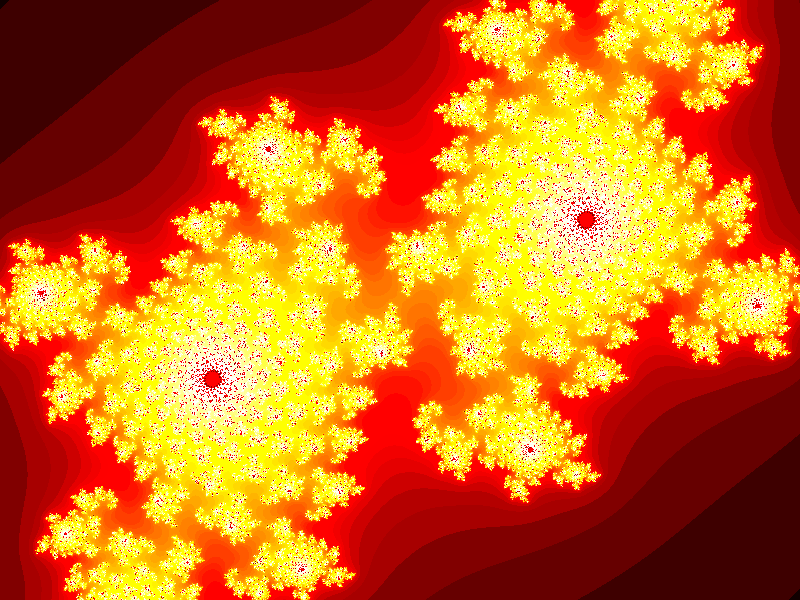
\includegraphics[width=0.33\linewidth]{./img/julia2}
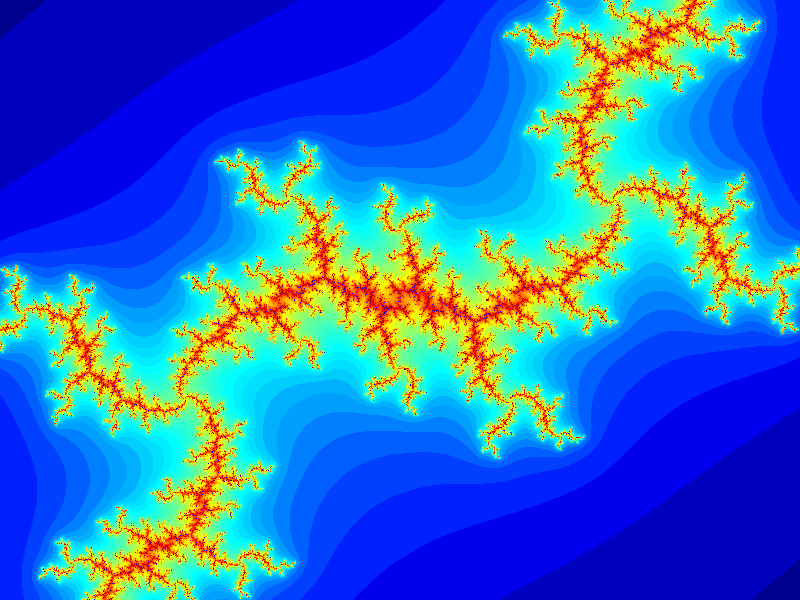
\includegraphics[width=0.33 \linewidth]{./img/julia4}
\caption{The Julia fractal shown using different seeds and colormaps.}
\label{fig:julia4}
\end{figure}
